Os modelos canônicos de CNNs são arquiteturas que trouxeram contribuições importantes, pioneiras na aplicação de técnicas que são comuns ainda hoje no cenário de DL, e que são comumente utilizadas em diversas tarefas de aprendizado \cite{9dlpapers}.

A LeNet é o primeiro modelo de rede neural a aplicar convoluções ao invés das camadas totalmente conectadas convencionais. Foi proposta por LeCun em 1998 e é composta de 7 camadas, sendo uma camada de entrada, duas camadas convolucionais, duas camadas de pooling, uma camada totalmente conectada e a camada de saída. A tarefa de aprendizado endereçada por esta rede na ocasião de sua proposição foi o reconhecimento de dígitos manuscritos. Para o treinamento e teste desta rede foi utilizado o conjunto de dados \emph{Modified National Institute of Standards and Technology} (MNIST), composto de 60000 imagens de treinamento e 10000 de teste dos dígitos de 0 a 9 escritos à mão. A LeNet foi amplamente utilizada por bancos para o reconhecimento de números escritos à mão em cheques digitalizado em imagens em escala de cinza de tamanho $32 \times 32$ \cite{lenet}. Apesar de pesquisas nesta área continuarem no decorrer dos anos, a quantidade insuficiente de bases de imagens catalogadas e o baixo poder computacional da época fizeram com que as CNNs permanecessem sem grandes destaques até o ano de 2012 \cite{dl9papers}.

AlexNet foi a primeira CNN ganhadora do desafio ILSVRC, em 2012, ao atingir um erro top-5 igual a $15.4\%$. O segundo melhor modelo daquele ano atingiu um erro de $26.2\%$. Esta rede, treinada para uma tarefa de classificação utilizando imagens de 1000 categorias da ImageNet, é formada por 5 camadas convolucionais com filtros de tamanho $11 \times 11$, intercaladas com camadas de \emph{max-pooling} e \emph{dropout} e $3$ camadas totalmente conectadas. Utilizava a função de ativação \emph{ReLU} ao invés da tradicional tangente hiperbólica. Na ocasião, para obter uma quantidade de exemplos razoável mediante o número de parâmetros ajustáveis, foi realizado um aumento artificial nas imagens de entrada, modificando-as segundo translações, reflexões horizontais e cortes. A AlexNet foi então treinada utilizando duas GPU GTX 580 por 5 a 6 dias, com o algoritmo de \emph{backpropagation} utilizando gradiente descendente estocástico para \emph{batch} e técnicas como \emph{momentum} e \emph{weight decay}. Estas técnicas garantiram à rede um desempenho significativamente melhor que o dos modelos tradicionais que estavam sendo aplicados para a ILSVRC daquele ano \cite{alexnet}.

Uma CNN que com um amplo destaque pela simplicidade e profundidade é a VGG. Apesar de não ter ganhado a ILSVRC 2014, alcançou um erro top-5 de $7.3\%$. Foi concebida na Universidade de Oxford, a VGG-19 contendo 19 camadas que utiliza estritamente filtros de $3 \times 3$ com \emph{stride} e \emph{pad} de 1, juntamente com \emph{max-pooling} de tamanho $2 \times 2$ e \emph{stride} 2. O número de filtros dobra após cada camada de \emph{max-pooling}, o que reforça a idéia de diminuir dimensões espaciais de largura e altura e aumentar a profundidade. A VGG-19 foi treinada em parte da base ImageNet utilizando 4 GPUs Nvidia Titan Black por duas a três semanas \cite{vggnet}.

Uma das primeiras arquiteturas de CNNs que se desviou do caminho normal de simplesmente empilhar camadas convolucionais e de pooling em uma estrutura sequencial foi a GoogLeNet, também chamada de Inception. Dotada de 22 camadas convolucionais, a rede ganhou o ILSVRC 2014 com um erro top-5 de $6.7\%$. Esta performance se deve aos chamados de módulos Inception, compostos de camadas da rede que ocorrem em paralelo. Ao invés de realizar uma operação de convolução ou \emph{max-pooling} de cada vez, várias operações diferentes são realizadas e os mapas de características obtidos são condensados e conectados ao próximo bloco Inception. A Figura \ref{fig:bloco_inception} mostra que há 4 conjuntos de operações a serem realizadas, todas contendo convoluções com filtros $1 \times 1$ em algum ponto, podendo haver também a convolução com filtros de tamanho $3 \times 3$, $5 \times 5$, ou uma operação de \emph{max-pooling} de $3\times 3$. A convolução com filtro $1\times 1$ é aplicada para reduzir a dimensionalidade do problema reduzindo a profundidade do mapa de características, além de retirar da entrada informações bem detalhadas em volume. As convoluções que utilizam filtros de $3\times 3$ e $5\times 5$ dão ao modelo a capacidade de extrair informações relevantes em larga escala. A camada de \emph{max-pooling} é aplicada a fim de reduzir a largura e altura do mapa de característas e combater \emph{overfitting}. Na GoogLeNet, as camadas totalmente conectadas são substituídas por \emph{average pooling}, o que economiza um grande número de parâmetros. A rede, que foi treinada em algumas GPUs de alta performance por uma semana, utiliza ReLU como função de ativação e dispõe de 9 módulos Inception com mais de 100 camadas no total. Todas estas técnicas utilizadas para reduzir a dimensionalidade do problema surtiram efeito pois, como mostrado na Figura \ref{fig:compara_redes},  nota-se que esta rede tem 12 vezes menos parâmetros que a sua predecessora AlexNet \cite{inception}.

\begin{figure}[h!]
	\centering
	\caption{Bloco Inception da CNN GoogLeNet. Fonte: \cite{9dlpapers}.}
	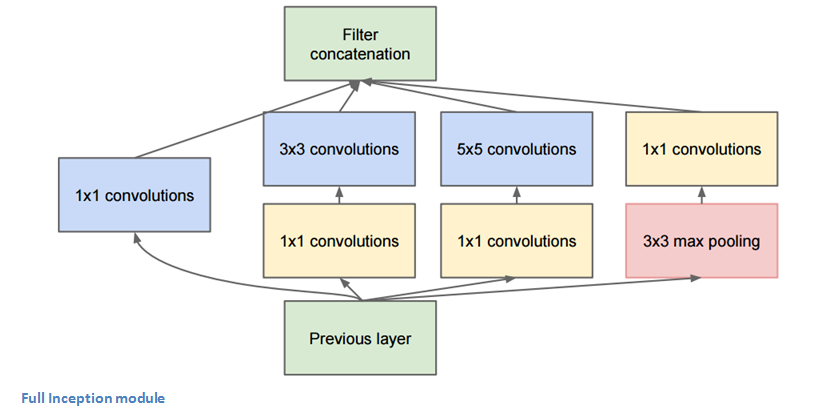
\includegraphics[width=0.7\linewidth]{img/GoogLeNet}
	\label{fig:bloco_inception}
\end{figure}



A Microsoft ResNet foi a CNN vencedora do ILSVRC 2015, com uma taxa de erro top-5 de $3.6\%$. Composta de um total de 152 camadas, esta rede neural deve o sucesso de sua profundidade ao bloco residual, representado na Figura \ref{fig:bloco_residual} que, de maneira resumida, soma à saída de um certo bloco de convoluções a saída de um bloco anterior, para que ambos \emph{feature maps} sejam alimentados à função de ativação ReLU. \todo{A imagem não está boa pq tem informações que não estão no texto.}

\begin{figure}[h!]
\centering
\caption{Bloco Residual da CNN ResNet. Fonte: \cite{torch:resnet}.}\label{fig:bloco_residual}
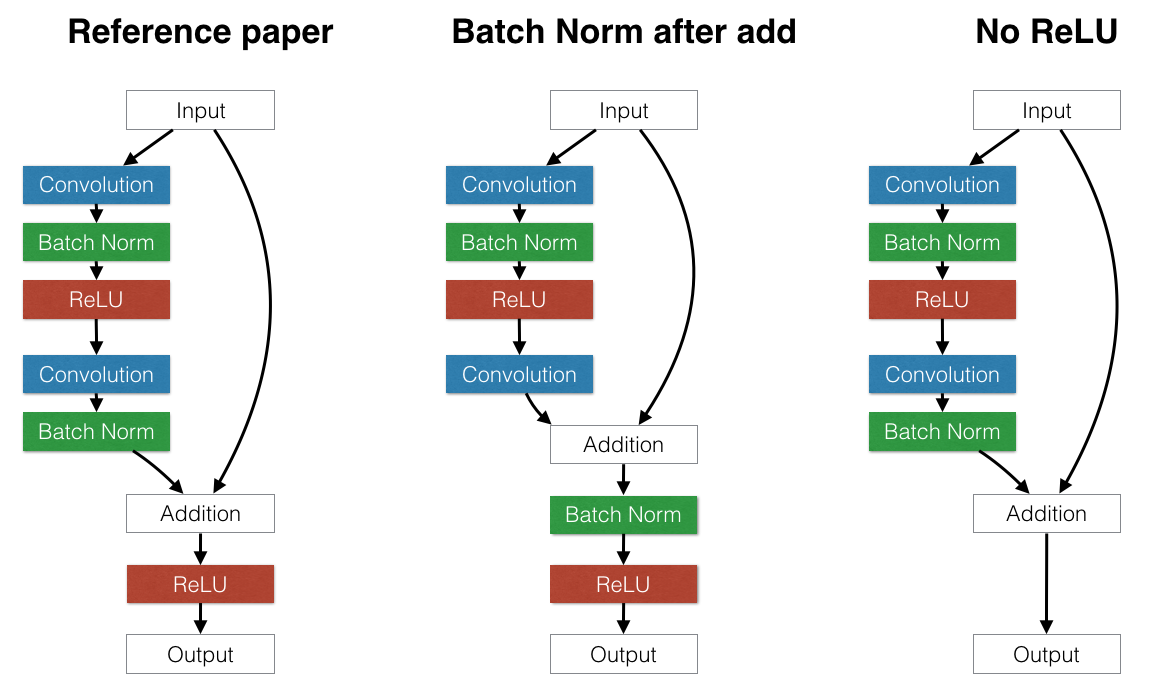
\includegraphics[width=0.7\linewidth]{img/resnets_modelvariants}
\end{figure}

Em CNNs tradicionais, a partir de uma imagem de entrada, obtém-se o  \emph{feature map}  resultante de uma operação de convolução e então aplica-se o \emph{max-pooling}. Este resultado produz uma nova representação, a qual possui pouca relação com a entrada original. No caso da ResNet, o bloco residual faz com que a entrada original persista em camadas mais profundas da rede, o que garante que as características determinantes para a tarefa de aprendizado sejam disseminadas para camadas mais profundas, ao mesmo tempo em que mantém a dimensionalidade reduzida. Outra razão para o bloco residual ser efetivo é que durante a fase \emph{backwards} o gradiente vai fluir mais facilmente pela rede, pois os blocos residuais estão diretamente conectados às camadas mais rasas na arquitetura, o que facilita a distribuição do gradiente. Na ocasião da sua proposição, a ResNet foi treinada em 8 GPUs por duas a três semanas. \todo{Falta citação da ResNet}

Observada a importância das CNNs apresentadas nesta seção, vale notar o esforço computacional para o treino das mesmas, que demora dias mesmo com um hardware específico para este fim. Todo o resultado do treinamento destas redes com o conjunto de dados ImageNet encontram-se disponíveis em \emph{frameworks} para implementação de CNNs, como o  \emph{Keras} \cite{keras:applications} e \emph{Tensorflow} \cite{tensorflow:models}. Disponibilizar estas versões de tais CNNs favorece o aproveitamento das mesmas em contextos análogos, como mostrado a seguir.
